\documentclass[paper=a4, 	% Seitenformat
		fontsize=11pt, 		% Schriftgr\"o\ss{}e
 		bibtotoc, 	% Literaturverzeichnis in das Inhaltsverzeichnis
% 		bibtotocnumbered, % Literaturverzeichnis mit Nummer in das Inhaltsverzeichnis
%		twoside, 	% doppelseitig
% 		idxtotoc, 	% Index in das Inhaltsverzeichnis
		abstracton, 	% mit Abstrakt
		headsepline, 	% Trennlinie f\"ur die Kopfzeile
		%footnosepline,	% Trennlinie f\"ur die Fu\ss{}zeile
		notitlepage	% keine extra Titelseite
		]{scrartcl}
%------------------------------------------------------------------------


%-----------------------------------------------------------------------------------
% zweiseitige Kopf-Zeilen
%-----------------------------------------------------------------------------------

\usepackage[automark]{scrpage2}	% Seiten-Stil f\"ur scrartcl
\pagestyle{scrheadings}		% Kopfzeilen nach scr-Standard
\ifx\chapter\undefined 		% falls Kapitel nicht definiert sind
  \automark[subsection]{section}% Kopf- und Fusszeilen setzen
\else				% Kapitel sind definiert
  \automark[section]{chapter}	% Kopf- und Fusszeilen setzen
\fi

%-----------------------------------------------------------------------------------
%   Maske f\"ur \"Uberschrift
%-----------------------------------------------------------------------------------
% Belegung der notwendigen Kommandos f\"ur die Titelseite
\newcommand{\autor}{Christoph Biesinger} 		% bearbeitender Student
\newcommand{\veranstaltung}{Projektmodul} 	% Titel des ganzen Seminars
\newcommand{\uni}{Institut f\"ur Informatik der Universit\"at Augsburg} % Universit\"at
\newcommand{\lehrstuhl}{Kommunikationssysteme} % Lehrstuhl
\newcommand{\semester}{}	% Winter- oder Sommersemester mit Jahr
\newcommand{\datum}{} 			% Datumsabgabe
\newcommand{\thema}{Analyse und Anwendung des Entwicklungsrepository ns-3-dev-TSCH}  		% Titel der Seminararbeit

\newcommand{\ownline}{\vspace{.7em}\hrule\vspace{.7em}} % horizontale Linie mit Abstand

\newcommand{\seminarkopf}{	% Befehl zum Erzeugen der Titelseite f\"ur kleinere Arbeiten
				% wie Seminarausarbeiten und numerisches Praktikum
 \textsc{\autor}  \hfill{\datum} \\
\textbf{\veranstaltung} \\
\uni \\
\lehrstuhl \\
\semester
\ownline

\begin{center}
{\LARGE \textbf{\thema}}
\end{center}
\ownline\vspace{2em} \vspace{2em}
\noindent
\ownline

}
%-----------------------------------------------------------------------------------

%-----------------------------------------------------------------------------------
%   Maske f\"ur neuen Abschnitt
%   nur bei f\"ur besondere Nummerierung notwendig,
%   zum Beispiel wenn die Kapitelnummer nicht bei 1 starten soll
%-----------------------------------------------------------------------------------
\newcommand {\abschnitt} [2]		% \"Uberschriftenbefehl f\"ur eigene Nummerierungen
{\setcounter{section}{#1}
 \setcounter{theorem}{0}
 \setcounter{equation}{0}
 \vspace{4ex}
 {\large \textbf{#1. #2}}
\vspace{1ex}}


% -----
% Bilder
% -----
%\graphicspath{{./images/}}
			% Befehle und Pakete f\"ur Titel
% Mathematische Zeichens\"atze und Umgebungen
\usepackage{amsfonts, amssymb}	% Definition einer Liste mathematischer Fontbefehle und Symbole
\usepackage[intlimits,		% Integralgrenzen \"uber und unter dem Integral
	    sumlimits]		% Summationsgrenzen \"uber und unter der Summe
           {amsmath}		% mathematische Verbesserungen
\usepackage{amsthm}		% spezielle theorem Stile
\usepackage{aliascnt}
%\usepackage{ntheorem-hyper}

% Code
\usepackage{listings}
\usepackage{color}

\definecolor{mygreen}{rgb}{0,0.6,0}
\definecolor{mygray}{rgb}{0.5,0.5,0.5}
\definecolor{mymauve}{rgb}{0.58,0,0.82}

\usepackage{float}
\usepackage{listings}

\newfloat{lstfloat}{htbp}{lop}
\floatname{lstfloat}{Listing}

\lstset{ %
  backgroundcolor=\color{white},   % choose the background color; you must add \usepackage{color} or \usepackage{xcolor}
  basicstyle=\footnotesize,        % the size of the fonts that are used for the code
  breakatwhitespace=false,         % sets if automatic breaks should only happen at whitespace
  breaklines=true,                 % sets automatic line breaking
  captionpos=b,                    % sets the caption-position to bottom
  commentstyle=\color{mygreen},    % comment style
  deletekeywords={...},            % if you want to delete keywords from the given language
  escapeinside={\%*}{*)},          % if you want to add LaTeX within your code
  extendedchars=true,              % lets you use non-ASCII characters; for 8-bits encodings only, does not work with UTF-8
  frame=single,	                   % adds a frame around the code
  keepspaces=true,                 % keeps spaces in text, useful for keeping indentation of code (possibly needs columns=flexible)
  keywordstyle=\color{blue},       % keyword style
  language=c++,                 % the language of the code
  otherkeywords={*,...},           % if you want to add more keywords to the set
  numbers=left,                    % where to put the line-numbers; possible values are (none, left, right)
  numbersep=5pt,                   % how far the line-numbers are from the code
  numberstyle=\tiny\color{mygray}, % the style that is used for the line-numbers
  rulecolor=\color{black},         % if not set, the frame-color may be changed on line-breaks within not-black text (e.g. comments (green here))
  showspaces=false,                % show spaces everywhere adding particular underscores; it overrides 'showstringspaces'
  showstringspaces=false,          % underline spaces within strings only
  showtabs=false,                  % show tabs within strings adding particular underscores
  stepnumber=2,                    % the step between two line-numbers. If it's 1, each line will be numbered
  stringstyle=\color{mymauve},     % string literal style
  tabsize=2,	                   % sets default tabsize to 2 spaces
  title=\lstname                   % show the filename of files included with \lstinputlisting; also try caption instead of title
}

%-----------------------------------------------------------------------------------
% Hilfreiche Befehle
%-----------------------------------------------------------------------------------
\newcommand{\betrag}[1]{\lvert #1 \rvert}	        % Betrag
\newcommand{\norm}[1]{\lVert #1 \rVert}		        % Norm
\providecommand*{\Lfloor}{\left\lfloor}                 % gro\ss{}es Abrunden
\providecommand*{\Rfloor}{\right\rfloor}                % gro\ss{}es Abrunden
\providecommand*{\Floor}[1]{\Lfloor #1 \Rfloor}         % gro\ss{}es ganzes Abrunden
\providecommand*{\Ceil}[1]{\left\lceil #1 \right\rceil} % gro\ss{}es ganzes Aufrunden
\newcommand{\eins}{ \mathds{1} }                        % Einsvektor

\newcommand{\R}{\mathbb{R}}

\DeclareMathOperator{\e}{ex}
\DeclareMathOperator{\ma}{mate}
\DeclareMathOperator{\Ex}{Ex}

%-----------------------------------------------------------------------------------
%   Befehle f\"ur Nummerierung der Ergebnisse
%   fortlaufend innerhalb eines Abschnittes
%-----------------------------------------------------------------------------------
\theoremstyle{plain}            % normaler Stil
\newtheorem{theorem}{Theorem}[section]
% Lemma
\newaliascnt{lemma}{theorem}
\newtheorem{lemma}[lemma]{Lemma}
\aliascntresetthe{lemma}
% Satz
\newaliascnt{satz}{theorem}
\newtheorem{satz}[satz]{Satz}
\aliascntresetthe{satz}
% Korollar
\newaliascnt{korollar}{theorem}
\newtheorem{korollar}[korollar]{Korollar}
\aliascntresetthe{korollar}
% Proposition
\newaliascnt{proposition}{theorem}
\newtheorem{proposition}[proposition]{Proposition}
\aliascntresetthe{proposition}
%-----------------------------------------------------------------------------------
\theoremstyle{definition}	% Definitionsstil
% Definition
\newaliascnt{definition}{theorem}
\newtheorem{definition}[definition]{Definition}
\aliascntresetthe{definition}
% Beispiel
\newaliascnt{beispiel} {theorem}
\newtheorem{beispiel}[beispiel]{Beispiel}
\aliascntresetthe{beispiel}
% Problem
\newaliascnt{problem}{theorem}
\newtheorem{problem}[problem]{Problem}
\aliascntresetthe{problem}
% Algorithmus
\newaliascnt{algorithmus}{theorem}
\newtheorem{algorithmus}[algorithmus]{Algorithmus}
\aliascntresetthe{algorithmus}
%-----------------------------------------------------------------------------------
\theoremstyle{remark}		% Bemerkungsstil
% Bemerkung
\newaliascnt{bemerkung}{theorem}
\newtheorem{bemerkung}[bemerkung]{Bemerkung}
\aliascntresetthe{bemerkung}
% Vermutung
\newaliascnt{vermutung}{theorem}
\newtheorem{vermutung}[vermutung]{Vermutung}
\aliascntresetthe{vermutung}
% Notation
\newaliascnt{notation}{theorem}
\newtheorem{notation}[notation]{Notation}
\aliascntresetthe{notation}

%-----------------------------------------------------------------------------------
% automatische Referenzen mit interaktiven Text
%-----------------------------------------------------------------------------------

% Texte
\newcommand{\theoremautorefname}{Theorem}
\newcommand{\lemmaautorefname}{Lemma}
\newcommand{\satzautorefname}{Satz}
\newcommand{\korollarautorefname}{Korollar}
\newcommand{\propositionautorefname}{Proposition}

\newcommand{\definitionautorefname}{Definition}
\newcommand{\beispielautorefname}{Beispiel}
\newcommand{\problemautorefname}{Problem}
\newcommand{\algorithmusautorefname}{Algorithmus}

\newcommand{\bemerkungautorefname}{Bemerkung}
\newcommand{\vermutungautorefname}{Vermutung}
\newcommand{\notationautorefname}{Notation}

%-----------------------------------------------------------------------------------
% Nummerierung der Gleichungen innerhalb der obersten Ebene
%-----------------------------------------------------------------------------------
\ifx\chapter\undefined 			% Kapitel sind definiert
  \numberwithin{equation}{section}	% Gleichungsnummern in Section
\else					% Kapitel sind nicht definiert
  \numberwithin{equation}{chapter}	% Gleichungsnummern in Kapiteln
\fi
			% Mathematische Befehle und Pakete
\usepackage{array}		% erweiterte Tabellen
\usepackage{alltt}

% Schriftzeichen, Format
\usepackage{latexsym}		% Latex-Symbole
\usepackage[latin1]{inputenc}	% Eingabekodierungen
\usepackage[english,ngerman]{babel}	% Mehrsprachenumgebung

% Layout
\usepackage{setspace}                   % Zeilenabstand
\usepackage{soul}                       % Unterstreichen mit Zeilenumbruch \ul{}
\usepackage{color}                      % Farben
\usepackage[right,official]{eurosym}    % Euro Symbol

% Bilder
\usepackage[final]{graphicx}            % Graphiken einbinden

\usepackage{caption}                    % Beschriftungen
\usepackage{subcaption}                 % Beschriftungen f\"ur Unterteilung
 \DeclareCaptionLabelFormat{contq}{#1~#2 (Fortsetzung)} % Fortgesetzte Umgebungen
 \captionsetup[ContinuedFloat]{labelformat=contq} % Fortgesetzte Umgebungen
 \captionsetup[longtable]{position=bottom}  % Beschriftungen unterhalb
 \captionsetup{format=hang}             % Platz unter dem Bezeichner und dem Trenner bleibt leer

%\psset{RightAngleType=german,comma=true} % Komma als Dezimalzeichen
% deutscher rechter Winkel


% Weitere Befehle
\newcommand{\gedanke}{-- }              % Gedankenstriche
\newcommand{\anfzeichen}[1]{"`#1"'}     % Anf\"uhrungszeichen
\newcommand{\define}[1]{\textit{#1}}    % Als neue Definition kennzeichnen
			% restliche Befehle und Pakete

% Literatur-Bibliothek
% \usepackage[authoryear]{natbib}              % Literaturangaben deutsch mit Autor und Jahr
% \bibliographystyle{alphadin}               % deutscher Bibliotheksstil
% \usepackage{csquotes}
% \usepackage[bibstyle=authoryear,
%             citestyle=authoryear-icomp,
%             backend=bibtex,
%             hyperref=auto,
%             backref=true,
%             clearlang=true,
%             language=german,
%             backrefstyle=three,
%             refsection=none, part, chapter, section, subsection
%             ]{biblatex}

 %Stil der Zitate und der Bibliographie
 \usepackage[style=numeric-comp]{biblatex}
 \nocite{*}
 %Bibliographie laden:
 \addbibresource{Header/literatur.bib}


% Interaktive Referenzen, und PDF-Keys
\usepackage{xr-hyper}
\usepackage[pagebackref,                % R\"uckreferenz im Literaturverzeichnis
           ps2pdf,                      % Treiber f\"ur ps zu pdf ; f\"ur direkt nach pdf: pdftex
           ]{hyperref}

% Erweiterte Einstellungen zu hyperref

\hypersetup{
        breaklinks=true,        % zu lange Links unterbrechen
        colorlinks=true,        % F\"arben von Referenzen
        citecolor=black,        % Farbe der Zitate
        linkcolor=black,        % Farbe der Links
         pagecolor=black,        % Farbe der Seitenlinks
        extension=pdf,          % Externe Dokumente k\"onnen eingebunden werden.
        %linktocpage,           % Seite im Inhaltsverzeichnis als Link nicht der Text
        ngerman,
	pdfview=FitH,
	pdfstartview=FitH,
	bookmarksnumbered=true, % Anzeige der Abschnittsnummern	% pdf-Titel
	pdfauthor={\autor}% pdf-Autor
}

% Namen f\"ur Referenzen

%\newcommand{\ownautorefnames}{
%  \renewcommand{\sectionautorefname}{Kapitel}
%  \renewcommand{\subsectionautorefname}{Unterkapitel}
%  \renewcommand{\subsubsectionautorefname}{\subsectionautorefname}
%  \renewcommand{\appendixautorefname}{Anhang}
%  \renewcommand{\figureautorefname}{Abbildung}
%}

% R\"uckreferenzentext zur Literatur
 % \renewcommand*{\bibbtasep}{, }
%\def\bibandname{und}%
%\renewcommand*{\backref}[1]{}
%\renewcommand*{\backrefalt}[4]{
%\ifcase #1 %(Nicht zitiert, also Erg\"anzungsliteratur.)
%\or %(Zitiert auf Seite #2.)
%\else %(Zitiert auf den Seiten #2.)
%\fi
%}
%\renewcommand{\backreftwosep}{ und~} % seperate 2 pages
%\renewcommand{\backreflastsep}{ und~} % seperate last of longer
			% restliche Befehle und Pakete

\numberwithin{figure}{section}	% Abbildungsnummern in Section

\begin{document}		% Start des Dokuments

\ownautorefnames		% \"Anderung einiger automatischen Texte von hyperref
\parindent0em 			% kein Einzug nach einer Leerzeile

\thispagestyle{empty}		% leerer Seitenstil, also keine Seitennummer

\begin{titlepage}
\seminarkopf 			% Titelblatt

\begin{abstract}
\section*{Kurzfassung}
Lorem ipsum dolor sit amet, consectetuer adipiscing elit, sed diam nonummy nibh euismod tincidunt ut laoreet dolore magna aliquam erat volutpat. Ut wisi enim ad minim veniam, quis nostrud exerci tation ullamcorper suscipit lobortis nisl ut aliquip ex ea commodo consequat. Duis autem vel eum iriure dolor in hendrerit in vulputate velit esse molestie consequat, vel illum dolore eu feugiat nulla facilisis at vero et accumsan et iusto odio dignissim qui blandit praesent luptatum zzril delenit augue duis dolore te feugait nulla facilisi. Nam liber tempor cum soluta nobis eleifend option congue nihil imperdiet doming id quod mazim placerat facer possim assum.
\end{abstract}


\end{titlepage}
				% \newpage streckt den Inhalt der aktuellen Seite auf die ganze Seite
\tableofcontents		% Inhaltsverzeichnis
%\listoffigures			% Abbildungsverzeichnis
%\listoftables			% Tabellenverzeichnis

\clearpage

\section{Grundlagen}
\label{sec:Grundlagen}
% ------------------------------------------------
% TSCH
% ------------------------------------------------
\subsection{IEEE 802.15.4e Timeslotted Channel Hopping}
\label{subsec:grundlagen_tsch}

\subsubsection{Time Divison Multiple Access TDMA}
\label{subsubsec:grundlagen_tdma}

\subsubsection{Enhanced Beacons und Information Elements}
\label{subsubsec:grundlagen_tsch_eb_ie}

\subsubsection{Network Formation Prozess}
\label{subsubsec:grundlagen_tsch_networkformation}
% ------------------------------------------------
% RPL
% ------------------------------------------------
\subsection{Routing Protocol for Low-Power and Lossy Networks RPL}
\label{subsec:grundlagen_rpl}

\subsubsection{Kontrollnachrichten}
\label{subsubsection:grundlagen_rpl_kontrollnachrichten}

DIO

\begin{lstlisting}[frame=single]
0                   1                   2                   3
0 1 2 3 4 5 6 7 8 9 0 1 2 3 4 5 6 7 8 9 0 1 2 3 4 5 6 7 8 9 0 1
+-+-+-+-+-+-+-+-+-+-+-+-+-+-+-+-+-+-+-+-+-+-+-+-+-+-+-+-+-+-+-+-+
| RPLInstanceID |Version Number |             Rank              |
+-+-+-+-+-+-+-+-+-+-+-+-+-+-+-+-+-+-+-+-+-+-+-+-+-+-+-+-+-+-+-+-+
|G|0| MOP | Prf |     DTSN      |     Flags     |   Reserved    |
+-+-+-+-+-+-+-+-+-+-+-+-+-+-+-+-+-+-+-+-+-+-+-+-+-+-+-+-+-+-+-+-+
|                                                               |
+                                                               +
|                                                               |
+                            DODAGID                            +
|                                                               |
+                                                               +
|                                                               |
+-+-+-+-+-+-+-+-+-+-+-+-+-+-+-+-+-+-+-+-+-+-+-+-+-+-+-+-+-+-+-+-+
|   Option(s)...
+-+-+-+-+-+-+-+-+
\end{lstlisting}

DAO

DIS

\subsubsection{Network Formation Prozess}
\label{subsubsec:grundlagen_rpl_networkformation}


% ------------------------------------------------
% Contik/Cooja
% ------------------------------------------------
\subsection{Contiki}
\label{subsec:grundlagen_contiki}

\subsubsection{Cooja}
\label{subsubsec:grundlagen_cooja}

\vspace{5em}

\section{Timeslotted Channel Hopping TSCH} \label{Kap5-4}

In diesem Kapitel werden nun die Funktionen und Eigenschaften des TSCH Mode
in der Theorie und dessen Implementierungsstand innerhalb von NS3 erl"autert.

Der Timeslotted Channel Hopping TSCH Mode ist haupts"achlich zur Unterst"utzung
von Anwendungen bei industrieller Automatisierung sowie Prozessmonitoring entwickelt
werden und charakterisiert sich dabei durch folgende Eigenschaften:

\begin{description}
  \item[Time Slotted Access] erh"oht den m"oglichen Datendurchsatz durch das
  Verhindern von Kollisionen zwischen in Wettbewerb stehenden Knoten und sorgt
  damit gleichzeitig f"ur eine vorhersagbare Latenz.
  \item[Multi-Channel Kommunikation] durch die Verwendung von mehreren "'Ubertragungskan"alen
  k"onnen mehrere Knoten zur gleichen Zeit (innerhalb des gleichen Zeitslots) senden,
  wodurch wiederum die Datendurchsatzkapazit"at gesteigert wird.
  \item[Channel Hopping] (auch Frequency Hopping) durch die verf"ugbaren "'Ubertragunskan"ale
  reduziert die Auswirkungen der Interferenz und Fading, wodurch die Kommunikation
  zuverl"assiger wird.
\end{description}

Daher wird eine erh"ohte Netzwerkauslastung und Zuverl"assigkeit garantiert
mit vorhersehbarer Latenz bei hoher Energieeffizienz, was zu einer Unabh"angigkeit
von Herstellern f"urht und besser f"ur Multi-Hop Netzwerke eignet.

% ----------------------------------------

\subsection{Time-slotted Access}

\subsubsection{Time Slots}
\label{sec:timeslots}

Timeslots sind klar definierte Zeitabschnitte, in denen ein Knoten agieren kann.
Dieser Zeitraum entspricht dabei dem im nachfolgenden Bild dargestellten Vorgang,
dem senden eines Pakets mit maximal m"oglicher Gr"osse (127 Byte) und dem Erhalt
der Antwort mittels ACK (1 ms) und dem \textit{packet processing} zur Verarbeitung
der Kommunikation (5 ms), wodurch ein Timeslot ca. 10ms lang ist.

\begin{figure}[h]
    \centering
    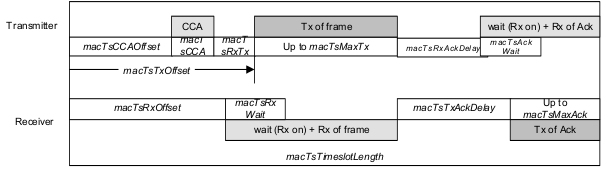
\includegraphics[scale=1.0]{images/timeslot.png}
    \caption{Timeslot \cite{IEEE802154e}}
    \label{fig:timeslot}
\end{figure}

Im aktuellen Entwicklungszustand, sind die Timeslots vollst"andig implementiert,
nachstehend die Datenstruktur f"ur die MacTimeslots in \textit{lr-wpan-tsch-mac.h}
in Zeile 146, welche der Abbildung \ref{fig:timeslot} entsprechen.
\begin{lstlisting}[frame=single]
typedef struct {
  //Table 52e TSCH-MAC PIB attributes for macTimeslotTemplate
  uint8_t m_macTimeslotTemplateId;
  uint16_t m_macTsCCAOffset;
  uint16_t m_macTsCCA;
  uint16_t m_macTsTxOffset;
  uint16_t m_macTsRxOffset;
  uint16_t m_macTsRxAckDelay;
  uint16_t m_macTsTxAckDelay;
  uint16_t m_macTsRxWait;
  uint16_t m_macTsAckWait;
  uint16_t m_macTsRxTx;
  uint16_t m_macTsMaxAck;
  uint16_t m_macTsMaxTx;
  uint16_t m_macTsTimeslotLength;
}LrWpanMacTimeslotTemplate;
\end{lstlisting}

\subsubsection{Slot Frames}
\label{sec:slotframes}

Slot Frames entstehen durch die Kombination mehreren Timeslots, welche sich
zyklisch wiederholen, wodurch sich die Knoten innerhalb des LR-WPANs miteinander
synchronisieren. Die Anzahl der Timeslots pro Slotframe Zyklus ist dabei variabel,
im nachfolgenden Beispiel sieht man ein Slotframe mit 4 Timeslots.

\begin{figure}[h]
    \centering
    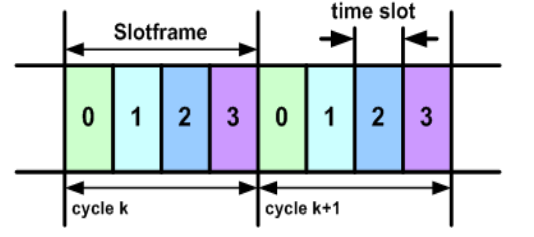
\includegraphics[scale=0.7]{images/slotframes.png}
    \caption{Slot Frames \cite{slotframes_fig}}
    \label{fig:slotframes}
\end{figure}

Auch die Slotframes sind vollst"andig implementiert. Als Beispiel die
Datenstruktur f"ur die Slotframe Operationen aus \textit{lr-wpan-tsch-mac.h}
in Zeile 202. Diese gibt die m"oglichen Operationen an, welche die MLME Schicht
(MAC Sublayer management entity) durchf"uhren kann. Namentlich, das hinzuf"ugen
und l"oschen einer Anzahl Slotframes bzw. das gezielte Modifizieren der
Slotframegr"osse.

\begin{lstlisting}[frame=single]
typedef enum {
  MlmeSlotframeOperation_ADD = 1,
  MlmeSlotframeOperation_DELETE = 2,
  MlmeSlotframeOperation_MODIFY = 3
}LrWpanMlmeSlotframeOperation;
\end{lstlisting}

% ----------------------------------------
\subsection{Multi-Channel communication}

\subsubsection{Node TSCH Schedule}

Unter dem TSCH Schedule eines Knoten wird die Frage beantwortet,
\textit{Was macht der Knoten innerhalb eines Timeslots?}
Ein Knoten kann dabei drei Aufgaben einnehmen, er kann als \textit{Transmit Slot}
ein Datenpaket senden und auf ein ACK warten, als \textit{Receive Slot} auf ein
Datenpaket warten und anschliessend ein ACK senden oder im Schlafmodus sein
und keine Aktion durchf"uhren.

In der Implementierung werden alle drei Aktionen innerhalb der Datei
\textit{lr-wpan-tsch-mac.cc} ab Zeile 1458 durchgef"uhrt in der Methode:

\begin{lstlisting}[frame=single]
void
LrWpanTschMac::ScheduleTimeslot(uint8_t handle, uint16_t size)
{
...
}
\end{lstlisting}

\begin{enumerate}
  \item Transmit Slot \hfill \\
    Ist f"ur einen Knoten ein Timeslot als Transmit Slot festgelegt, pr"uft
    dieser ob ein Paket im Buffer wartet, welches an den f"ur diesen Timeslot
    festgelegten Nachbarknoten vorgesehen ist. Sollte dies zutreffen wird das
    Paket gesendet, andernfalls gewartet bis der Nachbarknoten innerhalb eines
    Timeslot erreichbar ist.

    In der Implementierung kann das in \textit{lr-wpan-tsch-mac.cc} ab Zeile 1520
    nachverfolgt werden.

    \begin{lstlisting}[frame=single]
    if(m_macCCAEnabled)
      {
        Time time2wait = MicroSeconds(def_MacTimeslotTemplate.m_macTsCCAOffset);
        Simulator::Schedule(time2wait, &LrWpanTschMac::SetLrWpanMacState,this,TSCH_MAC_CCA);
        m_lrWpanMacStatePending = TSCH_MAC_CCA;
        Simulator::ScheduleNow(&LrWpanTschMac::SetLrWpanMacState,this,TSCH_MAC_IDLE);
      }
    else
      {
        Time time2wait = MicroSeconds(def_MacTimeslotTemplate.m_macTsTxOffset);
        Simulator::Schedule (time2wait,&LrWpanTschMac::SetLrWpanMacState,this,TSCH_MAC_SENDING);
        m_lrWpanMacStatePending = TSCH_MAC_SENDING;
        Simulator::ScheduleNow(&LrWpanTschMac::SetLrWpanMacState,this,TSCH_MAC_IDLE);
      }
    \end{lstlisting}

  \item Receive Slot \hfill \\
    Befindet sich ein Knoten im w"ahrend eines Timeslots im Receive Modus, wird dieser
    wie in Abbildung \ref{fig:timeslot} gezeigt f"ur einen definierten Zeitraum
    auf ankommende Frames und deren "'Ubermittelungszeit warten und nach einem
    erfolgreichen Erhalt des Frames ein passendes ACK-Frame zur"ucksenden, andernfalls
    wird der Knoten einfach bis zum Ende des Timeslots verweilen und nichts unternehmen.
    In der Implementierung ist das in \textit{lr-wpan-tsch-mac.cc} ab Zeile 1540 sichtbar.

    \begin{lstlisting}[frame=single]
    else if (it->macLinkOptions[1]) {
      //receive
      NS_LOG_DEBUG("Start timeslot receiving procedure");
      Time time2wait = MicroSeconds(def_MacTimeslotTemplate.m_macTsRxOffset);
      Simulator::Schedule (time2wait,&LrWpanTschMac::SetLrWpanMacState,this,TSCH_MAC_RX);
      m_lrWpanMacStatePending = TSCH_MAC_RX;
      Simulator::ScheduleNow(&LrWpanTschMac::SetLrWpanMacState,this,TSCH_MAC_IDLE);
      }
    \end{lstlisting}
\end{enumerate}

Damit ergibt sich ein Muster wie die Kommunikation zwischen den Knoten stattfindet,
was im Bild \ref{fig:tsch_link} exemplarisch dargestellt wird.

\begin{figure}[h]
    \centering
    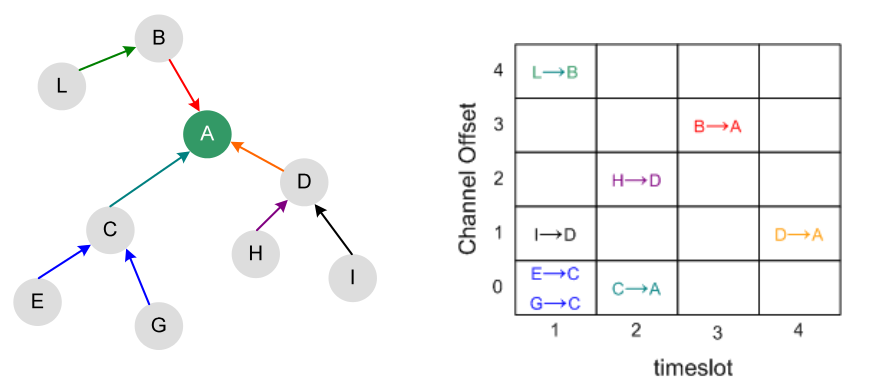
\includegraphics[scale=0.6]{images/tsch_link.png}
    \caption{TSCH Link \cite{tsch_link_fig}}
    \label{fig:tsch_link}
\end{figure}

% ----------------------------------------

\subsection{Frequency Hopping}

\subsubsection{Absolute Slot Number ASN}

Die Absolute Slot Number ASN, gibt an wie viele Timeslots seit dem Beginn des
Netzwerkes durchlaufen wurden. Damit k"onnen sich die Knoten untereinander
synchronisieren und neue neue Knoten dem Netzwerk beitreten (n"aheres dazu im
Kapitel Network Formation Process). Alle Knoten innerhalb des Netzwerkes kennen
zu jedem Zeitpunkt die global eindeutige ASN, welche deshalb f"ur zeitkritische
Anwendungen verwendet wird und zur Berechnung des Frequenzhoppings.
Zum Beginn des Netzwerkes wird die ASN auf den Wert 0 instanziiert und anschliessend
nach jedem Timeslot inkrementiert. Dies kann auch in der Implementierung in
\textit{lr-wpan-tsch-mac.cc} ab Zeile 1408 erkannt werden.

\begin{lstlisting}[frame=single]
void
LrWpanTschMac::IncAsn()
{
  NS_LOG_FUNCTION (this);
  m_newSlot = 1;
  m_macTschPIBAttributes.m_macASN++;
  Simulator::Schedule (MicroSeconds(def_MacTimeslotTemplate.m_macTsTimeslotLength),&LrWpanTschMac::IncAsn,this);
  ...
}
\end{lstlisting}

W"ahrend des laufenden Netzwerkes kann die ASN mit folgenden Formel nachberechent
werden, wobei \textit{k} der fortlaufende Slotframezyklus ist, \textit{S}
die Slotframegr"osse angibt und \textit{t} den SlotOffset beschreibt.
\begin{equation}
ASN = ( k * S + t)
\end{equation}

\subsubsection{Channel Hopping}

Die ASN wird insbesondere f"ur das Channel Hopping angewendet, wodurch ein Knoten
am Anfang bzw. Ende eines Timeslots seinen physikalischen Kommunikationskanal
wechselt. Da dieser Vorgang dauerhaft wiederholt wird und nur eine begrenzte Anzahl
an verf"ugbaren Kan"alen zur Verf"gung stehen \textit{springt} der Knoten zwischen
den Kan"alen hin und her.
Die Intention hinter dem Channel Hopping liegt darin begr"undet, dass in jedem
Slotframe ein anderer Kanal im jeweilig gleichen Timeslot angewendet wird.

Die Umsetzung dieses Kanalsprungverfahren wird durch folgende Formel bewerkstelligt,

\begin{equation}
Frequenz = F[ (ASN + channelOffset) \bmod nFreq]
\end{equation}

wobei \textit{F} eine Lookup Tabelle entspricht mit allen verf"ugbaren Frequenzen und
\textit{nFreq} die Anzahl der Frequenzen ist (laut Standard maximal 16 Frequenzen).

Durch die sich st"andig "'andernde ASN wird sichergestellt, dass nach jedem Slotframe
ein anderer Kanal berechnet wird und somit bildhaft durch die Frequenzen gesprungen
wird.

In der Abbildung \ref{fig:frequency_translation} wird gezeigt wie f"ur den gleichen
Timeslot (3) jeweils ein anderer Kanal berechnet wird. Das Channel Hopping ist auch
vollst"andig in ns3 implementiert, wie im nachfolgenden Codesnippet aus
\textit{lr-wpan-tsch-mac.cc} in der Methode \textit{LrWpanTschMac::ScheduleTimeslot}
in Zeile 1458 deutlich wird.

\begin{figure}[h]
    \centering
    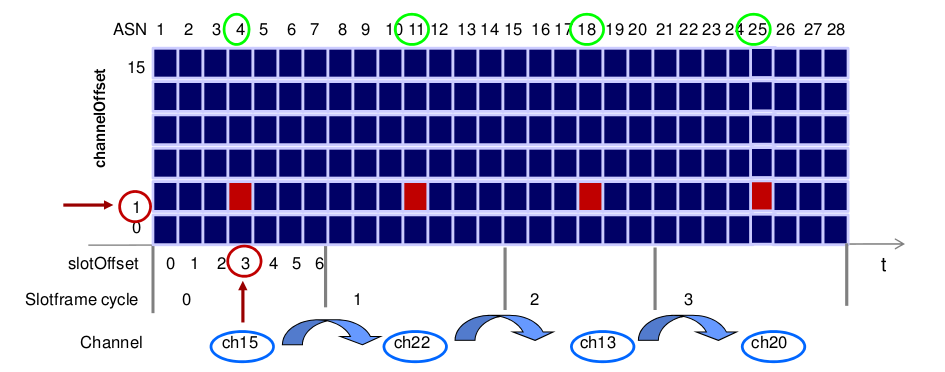
\includegraphics[scale=0.6]{images/frequency_translation.png}
    \caption{Channel Hopping \cite{frequency_translation_fig}}
    \label{fig:frequency_translation}
\end{figure}

\begin{lstlisting}[frame=single]
if (m_macHoppingEnabled)
  {
    //Get next channel
    m_currentChannel = def_MacChannelHopping.m_macHoppingSequenceList[
      (m_macTschPIBAttributes.m_macASN+it->macChannelOffset) % def_MacChannelHopping.m_macHoppingSequenceLength
      ];
}
\end{lstlisting}

\subsection{Time Synchronisation}

Die Kommunikation innerhalb von TSCH PAN verl"auft immer innerhalb von Timeslots,
weshalb eine Synchronisation zwischen den beteiligten Knoten umbedingt ben"otigt wird.
Um diese Synchronisation zu gew"ahrleisten m"ussen dabei alle Knoten den Beginn
das Ende der Timeslots kennen. Um dies Umzusetzen muss sich jedes Ger"at mit
mindestens einem anderen Ger"at innerhalb des PAN synchronisieren. Diese
Sychronisation erfolgt dabei im Regelfall vom PAN-Coordinator ausgehend durch das
gesamte Netzwerk und wird in der Abbildung \ref{fig:pan_synchronisation} exemplarisch
dargestellt. Dabei bedeutet ein Pfeil, dass der Zielknoten sich am ausgehenden
Knoten sychronisiert. Im Beispiel synchronisiert sich Device 2 mit Ger"at 1 und
dem PAN-Coordinator.

Die n"otigen Timing Informationen werden dabei in den normalen Daten und ACK
Paketen gesendet, welche innerhalb eines Time Correction Information Element
enthalten sind (mehr Informationen zu den Informationen Elements in Kapitel \ref{subsec:IE}).
Daher kann bei der Node Synchronisation auf zwei Arten unterschieden werden.

\begin{itemize}
  \item Frame-basiert
  \item Acknowledgment-basiert
\end{itemize}

wobei in beiden F"allen der Zeitunterschied gemessen wird, wann das jeweilige
Synchronisations-Paket eintreffen soll mit dem tats"achlichen Zeitpunkt.

\begin{figure}[h]
    \centering
    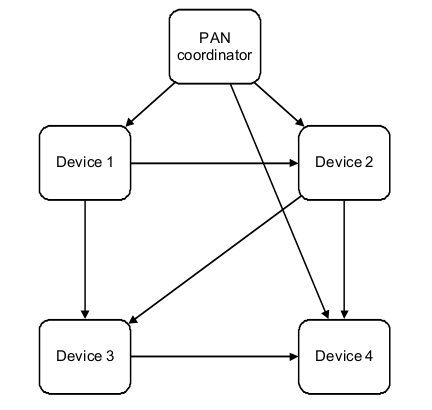
\includegraphics[scale=0.6]{images/pan_synchronisation.png}
    \caption{Beispielsynchronisation innerhalb eines PAN \cite{IEEE802154e}}
    \label{fig:pan_synchronisation}
\end{figure}

In ns3 fehlt eine aktive Implementierung eines Sychronisationsalgorithmus, da
innerhalb des Simulators alle Knoten auf den Beginn der Simulation synchronisiert
werden. In \textit{lr-wpan-tsch-mac.cc} Zeile 1368 kann beispielhaft gezeigt werden,
dass keine aktive Synchronisierung besteht.


\begin{lstlisting}[frame=single]
void
LrWpanTschMac::MlmeTschModeRequest (MlmeTschModeRequestParams params)
{
  NS_LOG_FUNCTION(this);
  MlmeTschModeConfirmParams confirmParams;
  confirmParams.TSCHMode = params.TSCHMode;

  switch(params.TSCHMode) {
    case MlmeTschMode_ON:

      /*TODO: Check if it is synced
      if (its not synced) {
        confirmParams.Status = LrWpanMlmeTschModeConfirmStatus_NO_SYNC;
      }*/
  }
}

\end{lstlisting}
% ----------------------------------------

\vspace{5em}

\section{Network Formation Process} \label{Kap5-5}

Dieses Kapitel beschreibt im Detail den Ablauf sowie die notwendigen Funktinalit"aten
f"ur den Network Formation Process eines IEEE 802.15.4e TSCH Netzwerkes.
Dabei wird zuerst das Konzept der Enhanced Beacons
EBs zur Informationsweiterleitung beschrieben mitsamt einem beispielhaften
Minimalaufbau, bevor der Network Formation Process anhand verschiedener
Sichtweisen erl"autert wird.

\subsection{Enhanced Beacons EB}

Enhanced Beacons EBs sind anwendungsbezogene Beacons, welche auf dem
Beacon Format beruhen und werden vor allem im DSME und TSCH Mode verwendet.
Sie bilden einen Mechanismus um Informationen aus h"oheren Schichten auch auf
der MAC Schicht zu nutzen. Erkenntlich werden EBs durch das \textit{Frame Version Field}
welches den Wert \textit{0b10} bekommt. Die gesendeten Informationen werden dabei
durch die Anbindung von Information Elements IE "ubermittelt.

Im TSCH Mode werden EBs vor allem angewendet um die Synchronisation der Knoten
innerhalb des PAN sicherzustellen, sowie im Network Formation Process.

\subsubsection{Information Elements IE}
\label{subsec:IE}

Information Elements IEs sind ein bekannter Mechanismus aus dem Standard IEEE
802.11 (WLAN) und sollen Informationen auf dem MAC Sublayer transportieren,
welche vorwiegend f"ur das Management des Netzwerkes dienen.

Man kann dabei zwischen zwei Arten an IEs unterscheiden,

\begin{description}
  \item[Header IE] sind Teil des MAC Headers und liefert Informationen damit der
  Media Access Control Layer das Frame verarbeiten kann.
  \item[Payload IE] wird innerhalb des MAC Payload gesendet und soll als
  Schnittstelle zu h"oheren Schichten dienen und Informationen weitergeben.
\end{description}

Der Aufbau von IEs ist dabei in beiden F"allen identisch, er beginnt mit dem
\textit{Type Descriptor} einem Flag von 1 Bit l"ange, welcher mit 0 ein Header IE
und mit 1 ein Payload IE angibt. Dannach folgt die 8 Bit lange \textit{Element ID}
um Angaben "'uber den Inhalt anzugeben, dem \textit{Length Field} mit 7 Bit und
abschliessend den 11 Bit langen \textit{Content}.

Der exemplarische Aufbau von IEs kann in der Implementierung in \textit{lr-wpan-mac-header.cc}
ab Zeile 1270 betrachtet werden. Die Anwendung dieser und spezielle IEs, gerade
f"ur den Network Formation Process, fehlen dagegen vollst"andig und m"ussen zur
weiteren Verwendung erst implementiert werden.

\begin{lstlisting}[frame=single]
//802.15.4 IE Header
if (m_fctrlFrmVer == 2 && m_fctrlIEListPresent == 1) {
  uint8_t lastid;

  do {
    HeaderIE* newie = new HeaderIE;
    uint16_t head = i.ReadLsbtohU16 ();
    newie->length = (head >> 9); //7 bits
    newie->id = (head >> 1); //8bits
    newie->type = 0; //1bit

    for (int j = 0;j<newie->length ;j++) {
      newie->content.push_back(i.ReadU8 ());
    }
    headerie.push_back(*newie);
    lastid = newie->id;
  } while (lastid != 0x7e && lastid != 0x7f);
}

\end{lstlisting}
\subsubsection{Minimaler Aufbau eines Enhanced Beacons}
\label{sec:Aufbau_Enhanced_Beacons}
Nachfolgend ist der Aufbau eines EB dargestellt, welcher minimal notwendig
ist um die Kommunikation mittels TSCH zu gew"ahrleisten.
Das Beispiel mitsamt der Erkl"arung ist dabei dem Internet-Draft
\href{https://tools.ietf.org/pdf/draft-ietf-6tisch-minimal-12.pdf#16}{6tisch-minimal}
entnommen.

\begin{lstlisting}[frame=single]
1                   2                   3
0 1 2 3 4 5 6 7 8 9 0 1 2 3 4 5 6 7 8 9 0 1 2 3 4 5 6 7 8 9 0 1
+-+-+-+-+-+-+-+-+-+-+-+-+-+-+-+-+-+-+-+-+-+-+-+-+-+-+-+-+-+-+-+-+
| Len1 =   0  |Element ID=0x7e|0|    Len2 = 26        |GrpId=1|1|
+-+-+-+-+-+-+-+-+-+-+-+-+-+-+-+-+-+-+-+-+-+-+-+-+-+-+-+-+-+-+-+-+
| Len3 =   6    |Sub ID = 0x1a|0|           ASN
+-+-+-+-+-+-+-+-+-+-+-+-+-+-+-+-+-+-+-+-+-+-+-+-+-+-+-+-+-+-+-+-+
              ASN                               | Join Priority |
+-+-+-+-+-+-+-+-+-+-+-+-+-+-+-+-+-+-+-+-+-+-+-+-+-+-+-+-+-+-+-+-+
|  Len4 = 0x01  |Sub ID = 0x1c|0| TT ID = 0x00  |   Len5 = 0x01
+-+-+-+-+-+-+-+-+-+-+-+-+-+-+-+-+-+-+-+-+-+-+-+-+-+-+-+-+-+-+-+-+
      |ID=0x9 |1| CH ID = 0x00  | Len6 = 0x0A   |Sub ID = 0x1b|0|
+-+-+-+-+-+-+-+-+-+-+-+-+-+-+-+-+-+-+-+-+-+-+-+-+-+-+-+-+-+-+-+-+
|   #SF = 0x01  | SF ID = 0x00  |   SF LEN = 0x65 (101 slots)   |
+-+-+-+-+-+-+-+-+-+-+-+-+-+-+-+-+-+-+-+-+-+-+-+-+-+-+-+-+-+-+-+-+
| #Links = 0x01 |      SLOT OFFSET = 0x0000     |    CHANNEL
+-+-+-+-+-+-+-+-+-+-+-+-+-+-+-+-+-+-+-+-+-+-+-+-+-+-+-+-+-+-+-+-+
  OFF  = 0x0000 |Link OPT = 0x0F|         NO MAC PAYLOAD
+-+-+-+-+-+-+-+-+-+-+-+-+-+-+-+-+
\end{lstlisting}

Der Aufbau entspricht dabei dem Header IE sowie dem Payload IE eines
Enhanced Beacons.

\begin{description}
  \item[Header IE Header] Len1 = Header IE L"ange, mit dem Wert 0,
  dem Element ID 0x7e, um anzuzeigen das sofort der Payload IE anschliesst,
  sowie dem Type mit Wert 0.
  \item[Payload IE Header] der Payload IE Header gibt mit \textit{Len2} seine
  L"ange mit 26 Byte an, der \textit{GroupID} von 1, was einem MLME Header entspricht
  sowie dem Type 1.
  \item[MLME-SubIE TSCH Synchronization] f"ur die Synchronisation wird mit
  \textit{Len3} ein 6 Byte langer Payload beschrieben, \textit{SubID} gibt
  den Wert \textit{0x1a} an, was f"ur einen MLME-SubIE TSCH Synchronization Header
  wirbt. Zus"atzlich kommt der \textit{Type} Short durch den Wert 0 zur anwendung,
  sowie der \textit{Absolut Sequence Number} mit einer L"ange von 5 Byte, sowie
  der \textit{Join Priority}.
  \item[MLME-SubIE TSCH TimeSlot] beschreibt die Timeslots beginnend mit
  \textit{Len4} von 1 Byte, der \textit{SubID} mit dem Wert \textit{0x1c} der
  das IE f"ur den Timeslot (MLME-SubIE Timeslote) angibt. Dazu wird der \textit{Type}
  als Short (0) sowie der standard \textit{Timeslot template ID} von \textit{0x00}
  angegeben.
  \item[MLME-SubIE Ch. Hopping] liefert die Informationen f"ur das Channel Hopping,
  mit \textit{Len5} einer L"angenfeld von 1 Byte, der \textit{SubID} von \textit{0x09}
  welche den Header als \textit{MLME-SubIE Ch. Hopping} ausgibt, dem \textit{type}
  und seinem Wert long (1), sowie der \textit{Channel Hopping Sequence ID}.
  \item[MLME-SubIE TSCH Slotframe and Link] der letzte IE liefert schliesslich
  die Informationen "'uber das TSCH Slotframe und dem sendenen Knoten.
  Beginnen mit der L"ange in Feld \textit{Len6} von 10 Byte, der \textit{SubID}
  mit Wert \textit{0x1b} der den Anwendungsfall des IE angibt (MLME-SubIE TSCH Slotframe and Link)
  einem \textit{type} von \textit{short} (0), der \textit{Number of slotframes} mit
  \textit{0x01}, dem \textit{SlotFrame Handle} mit Wert \textit{0x00}.
  Das \textit{SlotFrame Size} Feld liefert die Gr"osse von 101 Slots an (Wert von 0x65),
  gefolgt von der \textit{Number of Links}, dem aktuellen \textit{Timeslot},
  \textit{Channel Offset} und den \textit{Link Option} der mit dem Wert \textit{0x0F}
  die Optionen \textit{tx, rx, shared} und \textit{timekeeping} angibt.

\end{description}

% ----------------------------------------
\clearpage

\subsection{Network Formation Process}

Der Network Formation Process l"asst sich dabei in zwei Bereiche aufteilen. Das
"'Werben"' (Advertising) um neue Teilnehmer f"ur das Netzwerk, durch bereits im
Netzwerk befindliche Knoten, sowie einem "'Bootstrapping"'-Verfahren das ein Knoten
durchf"uhren muss um in das Netzwerk einzutreten. In der nachfolgenden Abbildung
\ref{fig:network_formation} wird der Prozess in einem Kontrollflussgraphen dargestellt.

\begin{figure}[h]
    \centering
    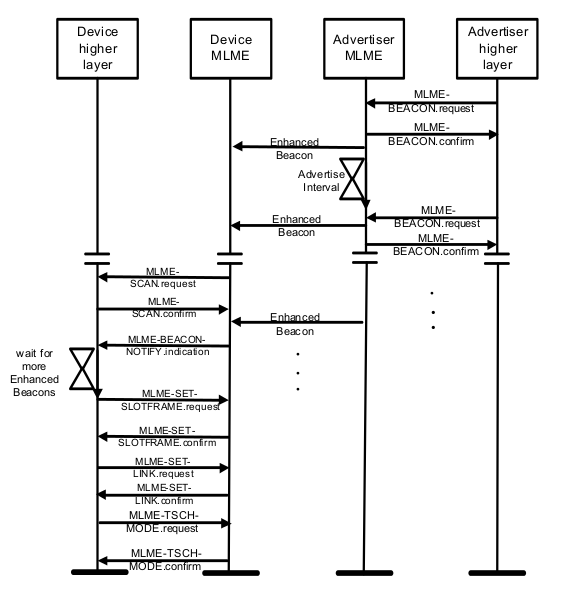
\includegraphics[scale=0.8]{images/tsch_advertisment.png}
    \caption{TSCH Prozedur f"ur Enhanced Beacons \cite{IEEE802154e}}
    \label{fig:network_formation}
\end{figure}

\clearpage
\subsubsection{Advertising}

Ein Personal Area Network PAN wird erstellt, indem ein Ger"at, in der Regel
der PAN-Coordinator die Existenz des Netzwerkes bekannt gibt. Dies geschieht
durch das Aussenden von Enhanced Beacons, welche Informationen innerhalb
von Information Elements enthalten
damit Knoten sich zum PAN synchronisieren k"onnen. Wie in Abbildung \ref{fig:network_formation}
abgebildet, beginnt das "'Werben"' indem ein \textit{MLME-BEACON.request} aus
einer h"oheren Schicht die Initiative gibt, Enhanced Beacons zu senden, welches
regelm"assig wiederholt wird.

Die enthaltenen Informationen der Enhanced Beacons, wurden konkret bereits im
vorherigen Kapitel beschrieben und enthalten:

\begin{itemize}
  \item Zeit Informationen, damit Knoten sich zum PAN synchronisieren k"onnen.
  \item Channel Hopping Informationen
  \item Timeslot Informationen, um zu erfahren wann Knoten als Receiver arbeiten
  um Frames zu empfangen und Acknowledgments zu senden.
  \item Initial Link- und Slotframe Informationen, "'ubermitteln die Informationen
  damit ein neuer Knoten weiss, wann er auf ankommende Verbindungen h"oren soll
  und wann er selber an seinen Advertisment Knoten senden kann.

\end{itemize}



Im aktuellen Entwicklungsstand wird deutlich, dass die ben"otigten IEs weder
vollst"andig implementiert sind noch deren gebrauch eingebettet ist. Als Beispiel
kann die Methode \textit{McpsDataRequest} aus dem Modul \textit{lr-wpan-tsch-mac.cc}
ab Zeile 241 gezeigt werden.

\begin{lstlisting}[frame=single]
void
LrWpanTschMac::McpsDataRequest (TschMcpsDataRequestParams params, Ptr<Packet> p)
{
...
if (params.m_frameControlOptions.IesIncluded)
  {
    macHdr.SetIEField();
    //TODO: Insert IEs
  }
else
  {
    macHdr.SetNoIEField();
  }
...
}
\end{lstlisting}

% ------------------------------------------------------------------------------
\subsubsection{"'Bootstrapping"'}

Der "'Bootstrapping"'-Algorithmus beschreibt das Verhalten von Knoten ausserhalb
des PAN und deren Aktivit"aten diesem beizutreten.

Wie in Abbildung \ref{fig:network_formation} gezeigt, wird der Knoten nach dem
Erhalt der Primitive \textit{MLME-SCAN.request} nach ankommenden EBs auf mehreren
Frequenzen suchen. Dadurch erh"alt der Knoten die notwendigen Informationen
indem er diese aus den EBs extrahiert und nun mit dem PAN sychronisiert.
Im Detail wird der Knoten sich an die Attribute der Slotframes und Timeslots anpassen,
da er sowohl die ASN wie auch die Timing-Informationen aus den IEs erhalten hat
um schlie"slich die Primitive \textit{MLME-SET-SLOTFRAME} zu aktivieren.
Anschliessend konfiguriert der Knoten seinen eigenen MLME Sublayer
mit \textit{MLME-SET-LINK} sowie dem aktivieren des TSCH Modes mit
\textit{MLME-TSCH-MODE} zur Kommunikation innerhalb des PAN.
Ist dieser Algorithmus abgeschlossen, ist der Knoten mit dem PAN innerhalb des
richtigen Slotframe und Timeslot synchronisiert und kann durch eigenst"andiges Senden
und Empfangen an diesem teilnehmen. Alle drei Primitiven sind vollst"andig im Modul
\textit{lr-wpan-tsch-mac.cc} implementiert.

\begin{itemize}
  \item MLME-SET-SLOTFRAME ist ab Zeile 1180 f"ur den Request implementiert.
    \begin{lstlisting}[frame=single]
      void
      LrWpanTschMac::MlmeSetSlotframeRequest (MlmeSetSlotframeRequestParams params)
      {
      ...
      }
    \end{lstlisting}
  \item Die Implementierung f"ur MLME-SET-LINK folgt ab Zeile 1258.
    \begin{lstlisting}[frame=single]
      void
      LrWpanTschMac::MlmeSetLinkRequest (MlmeSetLinkRequestParams params)
      {
      ...
      }
    \end{lstlisting}
  \item MLME-TSCH-MODE ab Zeile 1368 braucht noch die Abfrage der Synchronisation
    \begin{lstlisting}[frame=single]
      void
      LrWpanTschMac::MlmeTschModeRequest (MlmeTschModeRequestParams params)
      {
      ...
      }
    \end{lstlisting}
\end{itemize}

\vspace{5em}

\clearpage
\section{Kernfunktionalit"aten in der Entwicklung mit ns-3-dev-TSCH}

Dieses Kapitel beschreibt die Kernfunktionalit"aten welche f"ur den Umgang und
die Entwicklung mit dem Entwicklungsrepository ns-3-dev-TSCH wichtig sind.
Dabei werden zuerst die Kernmethoden aus der ns-3 Helperklasse
\textit{lr-wpan-tsch-helper} erl"autert, bevor weitere allgemeine ns-3
Funktionen n"aher betrachtet werden.

\subsection{Kernmethoden der Helperklasse LrWpanTschHelper}

\subsubsection{LrWpanTschHelper::Install}
Die Methode \textit{LrWpanTschHelper::Install} ab Zeile 309 enh"alt einen
NodeIterator welcher f"ur jeden erstellten Knoten das dazugeh"orige NetDevice
erstellt und ihm den richtigen Channel zuordnet. Wie im Kommentar ersichtlich
fehlt bislang die M"oglichkeit den Adressenmodus sowie die PanID f"ur
die NetDevices bei Erstellung festzulegen, statt dessen muss dieser Vorgang
in einem zus"atzlichen Schritt durchgef"uhrt werden.

\begin{lstlisting}[frame=single]
NetDeviceContainer
LrWpanTschHelper::Install (NodeContainer c)
{
  NetDeviceContainer devices;
  for (NodeContainer::Iterator i = c.Begin (); i != c.End (); i++)
    {
      Ptr<Node> node = *i;

      Ptr<LrWpanTschNetDevice> netDevice = CreateObject<LrWpanTschNetDevice> ();
      netDevice->SetChannel (m_channel);
      node->AddDevice (netDevice);
      netDevice->SetNode (node);
      // \todo add the capability to change short address, extended
      // address and panId. Right now they are hardcoded in LrWpanTschMac::LrWpanTschMac ()
      devices.Add (netDevice);
    }
  return devices;
}
\end{lstlisting}

\subsubsection{LrWpanTschHelper::AssociateToPan}
\label{helper_associatetopan}
Die Methode \textit{LrWpanTschHelper::AssociateToPan} beginnend ab Zeile 390
durchl"auft alle erstellten NetDevices und legt deren PanId und ShortAdresse
f"ur den TSCH (NMAC) und Nicht-TSCH (OMAC) Mode fest. Diese Funktionalit"aten
sollten in jeweils eigene Methoden ausgelagert werden, im besonderen das
Festlegen der Adressen um die hardgecodete Implementierung zu ersetzen.

\begin{lstfloat}
\begin{lstlisting}[frame=single]
void
LrWpanTschHelper::AssociateToPan (NetDeviceContainer c, uint16_t panId)
{
  NetDeviceContainer devices;
  uint16_t id = 1;
  uint8_t idBuf[2];

  for (NetDeviceContainer::Iterator i = c.Begin (); i != c.End (); i++)
    {
      Ptr<LrWpanTschNetDevice> device = DynamicCast<LrWpanTschNetDevice> (*i);
      if (device)
        {
          idBuf[0] = (id >> 8) & 0xff;
          idBuf[1] = (id >> 0) & 0xff;
          Mac16Address address;
          address.CopyFrom (idBuf);

          device->GetOMac ()->SetPanId (panId);
          device->GetOMac ()->SetShortAddress (address);
          device->GetNMac ()->SetPanId (panId);
          device->GetNMac ()->SetShortAddress (address);
          id++;
        }
    }
  return;
}
\end{lstlisting}
\end{lstfloat}

\subsubsection{LrWpanTschHelper::ConfigureSlotframeAllToPan}

Die Methode \textit{LrWpanTschHelper::ConfigureSlotframeAllToPan} ab Zeile 1068
definiert den Schedule der Kommunikation, durch die Reihenfolge der
Link-Methoden \textit{AddLink}, \textit{AddAdvLink} und \textit{AddBcastLinks}.
Die Methode erstellt am Anfang eine Anzahl an Slotframes in Abh"angigkeit
zur Anzahl der NetDevices, Empty Timeslots sowie einem zus"atzlichen Broadcast
und der M"oglichkeit der bidirektionalen Verbindung. Anschliessend werden
ein Advertisment Link im Timeslot 0 hinzugef"ugt, der optionale Broadcast Link
sowie den Direktverbindung an beteiligten NetDevices in einfacher und bidirektionaler
Verbindung.
Diese Methode sowie deren verwendeten Helper-Methoden m"ussen "uberarbeitet
werden, damit ein selbstgew"ahlter Schedule mit definierten Variablen anwendbar ist,
ansonsten k"onnen nur die im Rahmen der Parameter entsprechend Kommunikationsabl"aufe
definiert werden.


\begin{lstlisting}[frame=single]
void
LrWpanTschHelper::ConfigureSlotframeAllToPan(NetDeviceContainer devs, int empty_timeslots, bool bidir, bool bcast)
{
  int size = (bcast ? 2 : 1) + (bidir ? 2 : 1)*(devs.GetN ()-1) + empty_timeslots;

  AddSlotframe(devs,m_slotframehandle,size);

  //Add links
  AddLinkParams alparams;
  alparams.slotframeHandle = m_slotframehandle;
  alparams.channelOffset = 0;

  alparams.linkHandle = 0;
  alparams.timeslot = 0;
  AddAdvLink (devs,0,alparams);

  if (bcast) {
	  alparams.linkHandle = 1;
	  alparams.timeslot = 1;
	  AddBcastLinks (devs,0,alparams);
  }

  uint16_t c=(bcast ? 2 : 1);

  for (u_int32_t i = 0; i < devs.GetN ()-1; i++,c++)
    {
      alparams.linkHandle = c;
      alparams.timeslot = c;
      AddLink(devs,i+1,0,alparams,false);
    }

  if (bidir)
    for (u_int32_t i = 0; i < devs.GetN ()-1; i++,c++)
    {
      alparams.linkHandle = c;
      alparams.timeslot = c;
      AddLink(devs,0,i+1,alparams,false);
    }
   m_slotframehandle++;
}
\end{lstlisting}

\subsubsection{LrWpanTschHelper::AddAdvLink und LrWpanTschHelper::AddBcastLinks}

Die beiden Methoden \textit{LrWpanTschHelper::AddAdvLink} in Zeile 868 und
\textit{LrWpanTschHelper::AddBcastLinks} in Zeile 904 beschreiben den
Advertisment- bzw. Broadcast-Link. Nachfolgend ist der Code f"ur den Advertisment
Link abgebildet. Der Unterschied zwischen beiden Linktypen liegt in der Verarbeitung
der Sende und Empfangsverbindung.
Der Broadcast Link erstellt MlmeSetLinkRequests an alle Knoten und sendet an die
Adresse \textit{ff:ff} w"ahrend der Transmitphase. Im Laufe der Receive Phase
h"ort er auf die Adresse \textit{ff:ff} und "'offnet Links an alle Knoten mit einem
weiteren MlmeSetLinkRequest. Im aktuellen Entwicklungsstand ist der Broadcast Link
nicht anwendbar, da s"aemtliche Links innerhalb des PANs in den Sendenmodus geschaltet werden
und auch diesen w"ahrend des Timeslots nicht verlassen, weshalb zwar Pakete gesendet
aber nicht empfangen werden k"onnen.
F"ur unseren Anwendungsfall soll dieser allerdings den "'Join Request"' eines
beitretenden Knoten beinhalten, weshalb die Implementierung ge"andert werden muss.
Da zumindest der PAN Koordinator die Pakete empfangen muss gehen wir in Zukunft
davon aus, dass der PAN Koordinator das erste NetDevice darstellt. Konkret wird k"unftig
nicht erste NetDevice nicht mehr in den Transmit Modus geschalten, indem die for-Schleife
erst mit dem zweiten NetDevice beginnt zu z"ahlen.

\begin{lstlisting}[frame=single]
//10000000 to transmit
linkRequest.linkOptions.reset();
linkRequest.linkOptions.set(0,1);
linkRequest.linkOptions.set(2,1);
linkRequest.linkType = MlmeSetLinkRequestlinkType_ADVERTISING;
linkRequest.nodeAddr = Mac16Address("ff:ff");
for ( u_int32_t i = 1;i < devs.GetN ();i++)
  {
        linkRequest.TxID = i;
        linkRequest.RxID = coordinatorPos;
        linkRequest.linkFadingBias = FadingBias[coordinatorPos][i];
        devs.Get(i)->GetObject<LrWpanTschNetDevice> ()->GetNMac()->MlmeSetLinkRequest (linkRequest);
  }
\end{lstlisting}

Der Advertisment Link dagegen sendet in der Transmit Phase ebenfalls an die
Adresse \textit{ff:ff}, erstellt aber nur einen MlmeSetLinkRequest an ein bestimmten
NetDevice. Im Verlauf der Receive Phase wird nur auf die Adresse des Senders
geh"ort und nur zu diesem ein Link aufgebaut.

Die Methode \textit{LrWpanTschHelper::AddAdvLink} wird f"ur den Network Formation
Process ben"otigt und erh"aelt in der Variable \textit{u\_int32\_t senderPos}
das beizutretende NetDevice.

Aufgrund der momentanen Implementierung, k"onnen wir den Broadcast Link leider
nicht f"ur Broadcast Transmits verwenden, weshalb der Advertisment Link
diese Aufgabe "'ubernehmen wird, solange dieser Umstand nicht ge"andert wird.


\begin{lstlisting}[frame=single]
void
LrWpanTschHelper::AddAdvLink(NetDeviceContainer devs,u_int32_t senderPos, AddLinkParams params)
{
  MlmeSetLinkRequestParams linkRequest;
  linkRequest.Operation = MlmeSetLinkRequestOperation_ADD_LINK;
  linkRequest.linkHandle = params.linkHandle;
  linkRequest.slotframeHandle = params.slotframeHandle;
  linkRequest.Timeslot = params.timeslot;
  linkRequest.ChannelOffset = params.channelOffset;

  //10000000 to transmit
  linkRequest.linkOptions.reset();
  linkRequest.linkOptions.set(0,1);
  linkRequest.linkType = MlmeSetLinkRequestlinkType_ADVERTISING;
  linkRequest.nodeAddr = Mac16Address("ff:ff");
  linkRequest.linkFadingBias = NULL;
  linkRequest.TxID = senderPos;
  linkRequest.RxID = 0;
  devs.Get(senderPos)->GetObject<LrWpanTschNetDevice> ()->GetNMac()->MlmeSetLinkRequest (linkRequest);

  //01010000 to receive
  linkRequest.linkOptions.reset();
  linkRequest.linkOptions.set(1,1);
  linkRequest.linkOptions.set(3,1);
  linkRequest.nodeAddr = Mac16Address::ConvertFrom(devs.Get(senderPos)->GetAddress());
  for ( u_int32_t i = 0;i < devs.GetN ();i++)
      if (i != senderPos) {
          linkRequest.linkFadingBias = FadingBias[i][senderPos];
          linkRequest.TxID = senderPos;
          linkRequest.RxID = i;
          devs.Get(i)->GetObject<LrWpanTschNetDevice> ()->GetNMac()->MlmeSetLinkRequest (linkRequest);
        }
}
\end{lstlisting}

\subsubsection{LrWpanTschHelper::GenerateTraffic}

Mit den bislang beschriebenen Hilfsmethoden wird der Schedule innerhalb des TSCH
Mode fest und entsprechen damit den M"oglichkeiten die h"ohere Schichten besitzen
um Routing und Datenverkehr zu beschreiben. Dadurch wird zwar vorgegeben wann und
wie die Kommunikation innerhalb eines PAN stattfindet, der eigentliche Austausch von
Paketen zwischen den Knoten wird aber von einer anderen Hilfsmethode geregelt.

Diese Funktionalit"at wird von der Methode \textit{LrWpanTschHelper::GenerateTraffic}
ab Zeile 1129 wiedergespiegelt. Dabei wird ein Simulator Schedule gestartet, welcher
einen Ablauf an zeitdiskreten Events beschreibt wodurch MAC-Frames zwischen dem
ausgew"ahlten NetDevice \textit{dev} und seinem Ziel \textit{dst} gesendet werden.
Die Parameter \textit{start} und \textit{duration} geben dabei die Gesamtl"ange
der Kommunikation an. Wichtig ist zus"atzlich der Parameter \textit{interval}, welcher
die zeitlichen Abst"ande zwischen zwei Events angibt. Die Gewichtung dieses Parameter
wird im

\begin{lstlisting}[frame=single]
void
LrWpanTschHelper::GenerateTraffic(Ptr<NetDevice> dev, Address dst, int packet_size, double start, double duration, double interval)
{
  double end = start+duration;
  Simulator::Schedule(Seconds(start),&LrWpanTschHelper::SendPacket,this,dev,dst,packet_size,interval,end);
}
\end{lstlisting}


\subsection{Logging und Tracing}

Das Logging in ns3 erm"oglicht genaue Informationen "'uber den genauen Ablauf
der Netzwerksimulation zu erhalten wird das Logging eingesetzt, damit k"onnen
genauere Informationen erhalten werden, als beim "'ublichen Tracing. Da die
Informationsf"ulle extrem ansteigt wurde f"ur die einzelnen Loggingkomponenten
eine Hilfsmethode geschrieben.

\begin{lstlisting}[frame=single]
void
LogComponents(bool phy, bool csmaca, bool diverse)
{
  LogComponentEnableAll (LOG_PREFIX_TIME);
  LogComponentEnableAll (LOG_PREFIX_FUNC);
  LogComponentEnable ("LrWpanTschMac", LOG_LEVEL_ALL);
  LogComponentEnable ("LrWpanTschNetDevice", LOG_LEVEL_ALL);
  if (phy)
  {
  LogComponentEnable ("LrWpanPhy", LOG_LEVEL_ALL);
  LogComponentEnable ("LrWpanSpectrumSignalParameters", LOG_LEVEL_ALL);
  LogComponentEnable ("LrWpanSpectrumValueHelper", LOG_LEVEL_ALL);
  }
  if (csmaca)
  {
  LogComponentEnable ("LrWpanCsmaCa", LOG_LEVEL_ALL);
  }
  if (diverse)
  {
  LogComponentEnable ("LrWpanErrorModel", LOG_LEVEL_ALL);
  LogComponentEnable ("LrWpanInterferenceHelper", LOG_LEVEL_ALL);
  }
}
\end{lstlisting}

Als Beispiel wird ein Ausschnitt herangezogen, der am Anfang eines neuen diskreten
Events steht und die TSCH Funktionalit"at der Simulation angibt.
Darin meldet zuerst das LrWpanTschNetDevice \textit{00:02}, dass Daten an das Ger"at
mit der MAC-Adresse \textit{02-02-00:01} gesendet werden. Nachdem die Primitiven
gesetzt wurden, inkrementieren zuerst alle Ger"ate iher ASN und geben ihre
Aktion in diesem Timeslot an. Im Beispiel empf"angt \textit{00:01} Daten und
richtet sich darauf ein, diese zu Empfangen. Das Ger"at \textit{00:02} erkennt ein
Paket in seiner Warteliste und startet die Sendeprozedur.

\begin{lstlisting}[frame=single]
0.02s LrWpanTschNetDevice:Send(0x14ee770, 0x14fd5f0, 02-02-00:01, 34525)
0.02s LrWpanTschNetDevice:GetMtu(0x14ee770)
0.02s [address 00:02] LrWpanTschMac:McpsDataRequest(0x14ee800, 0x14fd5f0)
0.02s [address 00:02] LrWpanTschMac:SetTxLinkQueue(0x14ee800)
0.02s [address 00:02] LrWpanTschMac:SetTxLinkQueue(): Enqueuing packet with SeqNum = 108 in queue with link sequence = 0
0.02s [address 00:01] LrWpanTschMac:IncAsn(0x14ec530)
0.02s [address 00:02] LrWpanTschMac:IncAsn(0x14ee800)
0.02s [address 00:03] LrWpanTschMac:IncAsn(0x14f0c50)
0.02s [address 00:04] LrWpanTschMac:IncAsn(0x14f3080)
0.02s [address 00:05] LrWpanTschMac:IncAsn(0x14f54e0)
0.02s [address 00:06] LrWpanTschMac:IncAsn(0x14f7980)
0.02s [address 00:07] LrWpanTschMac:IncAsn(0x14f9da0)
0.02s [address 00:08] LrWpanTschMac:IncAsn(0x14fc1f0)
0.02s [address 00:01] LrWpanTschMac:ScheduleTimeslot(): Timeslot 2 ts = 2 Queue size = 0
0.02s [address 00:01] LrWpanTschMac:ScheduleTimeslot(): Link found at timeslot 2
0.02s [address 00:01] LrWpanTschMac:ScheduleTimeslot(): TSCH Changing to channel 18
0.02s [address 00:01] LrWpanTschMac:ScheduleTimeslot(): 0x14ec530setting for channel 18 fading bias: 1
0.02s [address 00:01] LrWpanTschMac:ScheduleTimeslot(): Start timeslot receiving procedure
0.02s [address 00:02] LrWpanTschMac:ScheduleTimeslot(): Timeslot 2 ts = 2 Queue size = 1
0.02s [address 00:02] LrWpanTschMac:ScheduleTimeslot(): Link found at timeslot 2
0.02s [address 00:02] LrWpanTschMac:ScheduleTimeslot(): TSCH Changing to channel 18
0.02s [address 00:02] LrWpanTschMac:ScheduleTimeslot(): 0x14ee800setting for channel 18 fading bias: 1
0.02s [address 00:02] LrWpanTschMac:ScheduleTimeslot(): Queue contained link size = 1
0.02s [address 00:02] LrWpanTschMac:FindTxPacketInEmptySlot(0x14ee800)
0.02s [address 00:02] LrWpanTschMac:FindTxPacketInEmptySlot(): Find Tx packet in queue with link position = 0 with queue size = 1
0.02s [address 00:02] LrWpanTschMac:ScheduleTimeslot(): Start timeslot transmiting procedure, seqnum = 108
0.02s [address 00:03] LrWpanTschMac:ScheduleTimeslot(): Timeslot 2 ts = 2 Queue size = 0
0.02s [address 00:03] LrWpanTschMac:ScheduleTimeslot(): No link in this timeslot, turning off the radio
0.02s [address 00:04] LrWpanTschMac:ScheduleTimeslot(): Timeslot 2 ts = 2 Queue size = 0
0.02s [address 00:04] LrWpanTschMac:ScheduleTimeslot(): No link in this timeslot, turning off the radio
0.02s [address 00:05] LrWpanTschMac:ScheduleTimeslot(): Timeslot 2 ts = 2 Queue size = 0
0.02s [address 00:05] LrWpanTschMac:ScheduleTimeslot(): No link in this timeslot, turning off the radio
0.02s [address 00:06] LrWpanTschMac:ScheduleTimeslot(): Timeslot 2 ts = 2 Queue size = 0
0.02s [address 00:06] LrWpanTschMac:ScheduleTimeslot(): No link in this timeslot, turning off the radio
0.02s [address 00:07] LrWpanTschMac:ScheduleTimeslot(): Timeslot 2 ts = 2 Queue size = 0
0.02s [address 00:07] LrWpanTschMac:ScheduleTimeslot(): No link in this timeslot, turning off the radio
0.02s [address 00:08] LrWpanTschMac:ScheduleTimeslot(): Timeslot 2 ts = 2 Queue size = 0
0.02s [address 00:08] LrWpanTschMac:ScheduleTimeslot(): No link in this timeslot, turning off the radio
\end{lstlisting}


Zum tracen der einzelnen Pakete, wird allen vorran die Methode \textit{EnablePcap}
verwendet um die pcap Dateien mitzuschneiden, welche anschliessend zur Netzwerkanalyse
in Wireshark ausgewertet werden k"onnen.
\begin{lstlisting}[frame=single]
lrWpanHelper.EnablePcap (std::string ("tsch_scenario"), panCoordNetDevice, true);
\end{lstlisting}

\vspace{5em}


\section{Experimente mit ns-3-dev-TSCH}

Zur Analyse des Codes und des k"unftigen Anwendungsfall wurden mehrere Beispielscripte
erstellt um verschiedene Aspekte zu analysieren, welche nachfolgend erl"autert werden.

\subsection{Kommunikation und Scheduling}

Als Grundlage und Kernaufgabe wurde die normale Kommunikation innerhalb des TSCH
Mode definiert, wobei an ein solch erstelltes PAN mehrere Anfoderungen festgelegt wurden.

\begin{itemize}
  \item Star bzw. Mesh TSCH Netzwerk,
  \item 7 FFDs und 1 PAN-Coordinator,
  \item Slotframe Size von 8, wobei der erste Slot f"ur das Senden der
  EBs vom PAN-Coordinator festgelegt wird,
  \item 100 Bytes an Daten pro gesendetem Paket von jedem der FFDs zum
  PAN-Coordinator, wobei eine Fragmentierung der Pakete vermieden werden soll,
  \item kein Network-Formation,
  \item und das Network Scheduling ist beliebig, wobei Kollisionen und Shared-Slots
  auch vermieden werden.
\end{itemize}

F"ur die Topologie ist das bereits im vorherigen Kapitel zum Thema Mobility vorgestellte
Codesnipped verantwortlich. Dabei wird ein Netzwerk aufgebaut, wobei alle 8 Knoten
anhand eines Grids auf zwei Reihen auf dem Koordinatensystem verteilt werden.

Wie im vorherigen Kapitel angeschnitten, definierten die Hilfsmethoden \textit{AddAdvLink},
\textit{AddLink} und \textit{AddBcastLinks} das Scheduling zwischen den Knoten
und die Methode \textit{GenerateTraffic} die tats"achliche Kommunikation.

Im Script wurde dabei zuerst die vorgegebene Hilfsmethode \textit{ConfigureSlotframeAllToPan}
mit unseren vorgegebenen Anfoderungen verwendet, welche folgenden Schedule vorgibt:

\begin{enumerate}
  \item Advertisment Link Dauer: 1 Timeslot
  \item Broadcast Link Dauer: 1 Timeslot
  \item Unidirektionale Verbindung zwischen den FFDs und dem PAN Koordinator 7 Timeslots
\end{enumerate}

Dieser Schedule mit einer Dauer von 9 Timeslots wird nun anschliessend f"ur die
Dauer des Scripts wiederholt. F"ur die tats"achliche Kommunikation ist nun das nachfolgende
Codesnipped verantwortlich, womit zuerst allgemein der PAN Koordinator an alle FFDs
ein Frame sendet und anschliessend in aneinanderfolgenden Timeslots jedes FFD sein
Frame an den PAN Koordinator sendet.

Ein wichtiger Unterschied muss erl"autert werden, zwischen dem Schedule eines Slotframes
im Gegensatz zur tats"achlichen Kommunikation zwischen den Knoten. Der Schedule umfasst
dabei einen vollen Slotframe und wird wiederholt und dauert wie im Beispiel angegeben
einen Zeitraum von 9 Timeslots. Die Kommunikation dagegen selber wird durch die
Methode \textit{LrWpanHelper::GenerateTraffic} vorgegeben, wodurch im Abstand von
vorgegeben Intervallzyklen, durch die Variable \textit{interval},
jeweils ein zeitdiskretes Event zum Senden der Frames festgelegt.


\begin{lstlisting}[frame=single]
// Packets from panCoord
Ptr<Node> panCoordNode = panCoord.Get (0);
Ptr<NetDevice> panCoordNetDevice = panCoordNode->GetDevice (0);
Address address_panCoord = panCoordNetDevice->GetAddress ();
//Broadcast address
Mac16Address brdcst ("ff:ff");
lrWpanHeelper.GenerateTraffic (panCoordNetDevice, brdcst, pktsize, 0.0, duration, interval);
// FFDs
for (NodeContainer::Iterator i = ffds.Begin (); i != ffds.End (); i++)
{
  Ptr<Node> node = *i;
  Ptr<NetDevice> device = node->GetDevice (0);
  lrWpanHelper.GenerateTraffic (device, address_panCoord, pktsize, starttopancoord, duration, interval);
  starttopancoord += 0.01;
}
\end{lstlisting}

% -----
\clearpage
\subsection{Script Kollision und Mobility}

Durch folgendes Script soll ermittelt werden wie sich der Entwicklungsstand bei
Kollisionen innerhalb des gleichen Timeslots verh"alt. Die daf"ur verwendete Topologie
besteht aus einem PAN Koordinator an welchen zwei FFDs im gleichen Timeslot "'uber
einen Shared Link diesem ein Paket senden womit es zum Kollisionsfall kommt.
Wie sich sp"ater herausstellt, beeinflusst die Position der Knoten zueinander das
Ergebnis.

Das Mobility Modul beschreibt die Position und Bewegung von Knoten im Netzwerk.
Die wichtigsten Einstellungen f"ur unseren Anwendungszweck sind dabei,

\begin{description}
  \item[Mobility Model] definiert die Bewegung von Knoten, wobei wir diese
  dauerhaft auf einer festen Position fixieren wollen. Daf"ur wird die Einstellung
  \textit{ns3::ConstantPositionMobilityModel} verwendet.
  \item [Position Allocator] setzt die (Start-)Position der Knoten fest. Dabei
  stehen mehrere Allokatoren zur Auswahl, wobei wir den \textit{ns3::GridPositionAlloctor}
  verwenden, der alle Knoten anhand eines Koordinatensystem mit festen Abst"anden
  zueinander erstellt
\end{description}

Als Vorlage zur Positionsfestlegung diente dabei folgendes Codesnipped:

\begin{lstlisting}[frame=single]
MobilityHelper mobility;
mobility.SetMobilityModel ("ns3::ConstantPositionMobilityModel");
mobility.SetPositionAllocator ("ns3::GridPositionAllocator",
                               "GridWidth", UintegerValue(2),
                               "MinX", DoubleValue (0.0),
                               "MinY", DoubleValue (0.0),
                               "DeltaX", DoubleValue (5),
                               "DeltaY", DoubleValue (5),
                               "LayoutType", StringValue ("RowFirst"));
mobility.Install (allNodes);
\end{lstlisting}

Daraus ergibt sich wie in nachfolgender Darstellung sichtbar, die Verteilung
der Knoten auf dem Grid, woran wir die Ergebnisse erl"autern.

\begin{lstlisting}[frame=single]
// FFD2 --
// PANC -- FFD1
\end{lstlisting}

\begin{description}
  \item[Unterschiedliche Entfernung der FFDs zum PAN Koordinator]
  Dieser Fall wird durch die Variablen \textit{DeltaX} und \textit{DeltaY} festgelegt,
  dabei zeigt das Ergebnis, dass beide FFDs nach einem erfolgreichen Clear Channel
  Assessment ihr Frame senden. Der PAN Koordinator akzeptiert aber nur das Frame
  dessen FFD das eine geringere Entfernung aufweist, da dieses eine gr"ossere
  Signalst"arke aufweist. Deshalb sendet der PAN Koordinator ein Ack-Frame mit der
  Sequenznummer des akzeptieren FFD. Im n"achsten Schritt empfangen beide FFDs dieses
  ACK-Frame und pr"ufen dessen Sequenznummer, wobei nur ein FFD dieses akzeptiert.
  Das andere FFD wird daraufhin im n"achsten m"oglichen Timeslot versuchen das
  somit abgelehnte Frame abermals zu senden, sobald der Backoff-Algorithmus dies zul"asst.
  \item[Gleiche Entfernung zueinander]
  Ein Sonderfall ergibt sich, wenn beide FFDs die selber Entfernung und somit die
  gleiche Signalst"arke zum PAN Koordinator aufweisen.
  Dabei wird zwar der gleiche Ablauf sichtbar, dass ein FFD erfolgreich
  sein Frame senden und das ACK-Frame empfangen und akzeptieren kann. Dieses FFD
  ist aber grunds"atzlich immer FFD Nummer 1. Dies wird durch die Implementierung
  von ns3 als diskreter Eventsimulator festgelegt, wobei ns3 iterativ alle Knoten pro
  Zeitpunkt durchl"auft und damit zuerst FFD1 berechnet.
\end{description}

Das Verhalten der Knoten nach einer solchen Kollision wird durch den weiteren
Schedule innerhalb des Slotframes festgelegt. Werden zus"atzliche dedizierte
Links zwischen den FFDs zum PAN Koordinator zu einem sp"ateren Timeslot innerhalb
des selben Slotframes festgelegt, wird das zum Kollisionszeitpunkt abgelehnte Frame
erfolgreich gesendet. Damit ist der TSCH CSMA-CA Backoff Algorithmus korrekt implementiert.

Fehlen diese dedizierten Links dagegen, wird das abgelehnte Frame erst im n"achsten Slotframe
gesendet und kann bei anhaltender Kollision f"ur einen langen Zeitraum blockiert werden,
womit alle in der Warteschlange befindlichen Frames des Knoten und damit dieser selber
blockiert.

Das allgemeine Verhalten im TSCH Mode wiederspricht aber den Vorgaben w"ahrend einer
Kollision, weshalb das Kollisionsverhalten mit der urspr"unglichen LRWPAN Version
ausserhalb des TSCH Mode verglichen wurde. Die Anforderungen und Vorraussetzungen sind
beibehalten worden.

Dabei zeigt sich das im normalen LRWPAN Modus im Kollisionsfall das Clear Channel
Assessment einem Knoten, in Abh"angigkeit von der Entfernung zum PAN Koordinator,
eine Backoffzeit zuteilt und diesen damit daran hindert sein Frame zu senden.
Damit wurde eine m"ogliche Kollision verhindert und die Kommunikation wird fortgesetzt.

Aufgrund diesen Vergleichs mit der normalen LRWPAN Version zeigt sich, dass das
Clear Channel Assessment im TSCH Mode Fehler aufweist, indem es im Kollisionsfall
nicht aktiv wird. Daf"ur wurde aber im Standard der TSCH CSMA-CA Backoff Algorithmus
eingef"uhrt, damit genau dieser Sonderfall behandelt werden kann. Wie Abbildung
\ref{fig:tsch_csma_backoff_algo} zeigt, wird im Kollisionsfall eine Backoffzeit
eingesetzt, in welcher der Knoten nicht versucht Frames zu senden obwohl der
Schedule aktive Links festgesetzt hat.
Da unsere Beispiele dieses Verhalten gezeigt haben, muss abschlie"send festgestellt
werden, dass das Kollisionsverhalten vollst"andig und korrekt implementiert ist.

\begin{figure}[h]
    \centering
    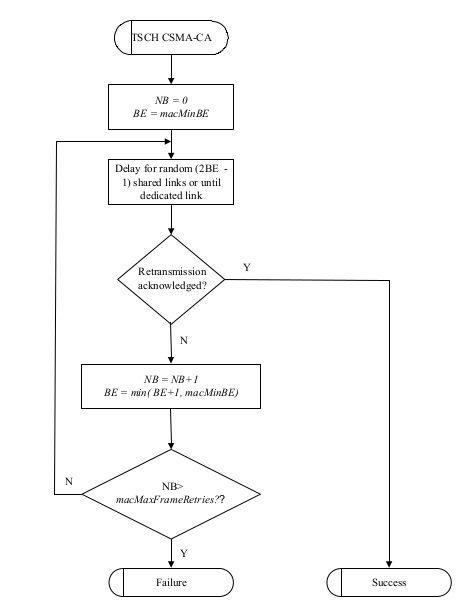
\includegraphics[scale=0.7]{images/tsch_csma_backoff_algo.png}
    \caption{TSCH CSMA-CA Backoff Algorithmus \cite{IEEE802154e}}
    \label{fig:tsch_csma_backoff_algo}
\end{figure}

\vspace{5em}

\section{Fazit und weiterf"uhrende Arbeiten} \label{Kap5-6}


\subsection{Grober Entwicklungsplan}

Anhand des Implementierungsstands m"ussen einige Entwicklungsarbeiten vorgenommen
werden, damit der Network Formation Process durchgef"uehrt werden kann. Nachfolgend
wird nun im Groben beschrieben was ein solcher Entwicklungsplan beinhaltet.

\begin{enumerate}
  \item Anpassen bzw. Neuentwicklung der Helpermethoden zur Erstellung
  von beliebigen Schedules mit beliebigen Variablenwerten f"ur Slotframes, Timeslots,
  ChannelOffset, SlotframeHandle mit den Linktypen Link, Advertisment Link und
  Broadcast Link.
  \item Analyse und Anpassung der aktuellen Grobstruktur der Information Elements
  \item Einbettung der IEs in die Module zur aktiven Anwendung
  \item Entwicklung von Helper Methoden zum Senden und Empfangen von IEs
  \item Helper Methoden und Einbettung der konkreten IEs innerhalb des Network
  Formation Process, wie in \ref{sec:Aufbau_Enhanced_Beacons} beschrieben
  \begin{itemize}
    \item Header IE Header
    \item Payload IE Header
    \item MLME-SubIE TSCH Synchronization
    \item MLME-SubIE TSCH Timeslot
    \item MLME-SubIE Channel Hopping
    \item MLME-SubIE TSCH Slotframe and Link
  \end{itemize}
  \item Beispiel zur Anwendung der IEs
  \item Implementierung des Advertisment Modes zum Aussenden der Enhanced Beacons
  \item Anpassen des "'Bootstrapping"'-Algorithmus anhand der neuen Implementierung.
\end{enumerate}

\vspace{5em}

\clearpage

%\appendix                       % Start des Anhangs

\section{Appendix: Scriptimplementierung}

\subsection{tsch\_scenario.cc}

\begin{lstlisting}[frame=single]
#include <ns3/log.h>
#include <ns3/core-module.h>
#include <ns3/network-module.h>
#include <ns3/lr-wpan-module.h>
#include <ns3/simulator.h>
#include <ns3/single-model-spectrum-channel.h>
#include <ns3/packet.h>
#include <ns3/mobility-module.h>
#include <ns3/spectrum-helper.h>
#include <string>

#include <iostream>

using namespace ns3;

/////////////////////////////////
// Configuration
/////////////////////////////////
bool verbose = true;       // enable logging
uint32_t numberOfFFDs = 7;      // FFDs
bool brdcst_as_join = true;
bool collision = true;

int pktsize = 91;           //size of packets, in bytes
double duration = 1;       //simulation total duration, in seconds
double starttopancoord = 0.02;        // Starttime transmitting FFDs
double interval = 0.2;
double starttoffds = 0.08;

void
LogComponents(bool phy, bool csmaca, bool diverse)
{
  LogComponentEnableAll (LOG_PREFIX_TIME);
  LogComponentEnableAll (LOG_PREFIX_FUNC);
  LogComponentEnable ("LrWpanTschMac", LOG_LEVEL_ALL);
  LogComponentEnable ("LrWpanTschNetDevice", LOG_LEVEL_ALL);
  if (phy)
  {
    LogComponentEnable ("LrWpanPhy", LOG_LEVEL_ALL);
    LogComponentEnable ("LrWpanSpectrumSignalParameters", LOG_LEVEL_ALL);
    LogComponentEnable ("LrWpanSpectrumValueHelper", LOG_LEVEL_ALL);
  }
  if (csmaca)
  {
    LogComponentEnable ("LrWpanCsmaCa", LOG_LEVEL_ALL);
  }
  if (diverse)
  {
    LogComponentEnable ("LrWpanErrorModel", LOG_LEVEL_ALL);
    LogComponentEnable ("LrWpanInterferenceHelper", LOG_LEVEL_ALL);
  }

}

void
EnableTsch(LrWpanTschHelper* lrWpanHelper,NetDeviceContainer& netdev)
{
  lrWpanHelper->EnableTsch(netdev,0,duration);
}

int main (int argc, char** argv)
{

  CommandLine cmd;
  cmd.AddValue ("verbose", "Print trace information if true", verbose);
  cmd.Parse (argc, argv);
  GlobalValue::Bind ("ChecksumEnabled", BooleanValue (true));

  // ----------------------------
  // Nodes
  NodeContainer ffds;
  NodeContainer panCoord;
  ffds.Create (numberOfFFDs);
  panCoord.Create (1);
  NodeContainer lrwpanNodes(panCoord, ffds);

  /////////////////////////////////
  // Mobility
  /////////////////////////////////

  MobilityHelper mobility;
  mobility.SetMobilityModel ("ns3::ConstantPositionMobilityModel");
  mobility.SetPositionAllocator ("ns3::GridPositionAllocator",
                                 "GridWidth", UintegerValue(4),
                                 "MinX", DoubleValue (0.0),
                                 "MinY", DoubleValue (0.0),
                                 "DeltaX", DoubleValue (5),
                                 "DeltaY", DoubleValue (5),
                                 "LayoutType", StringValue ("RowFirst"));
  mobility.Install (lrwpanNodes);

  /////////////////////////////////
  // Channel
  /////////////////////////////////
  SpectrumChannelHelper channelHelper = SpectrumChannelHelper::Default ();
  channelHelper.SetChannel ("ns3::MultiModelSpectrumChannel");
  Ptr<SpectrumChannel> channel = channelHelper.Create ();

  /////////////////////////////////
  // Configure lrwpan nodes
  /////////////////////////////////
  LrWpanTschHelper lrWpanHelper(channel,numberOfFFDs+1,false,true);

  // Add and install the LrWpanTschNetDevice for each node
  NetDeviceContainer netdev = lrWpanHelper.Install (lrwpanNodes);

  // AssociateToPan
  lrWpanHelper.AssociateToPan(netdev,123);

  // Slotframes
  lrWpanHelper.ConfigureSlotframeAllToPan(netdev,0,false,true); // slotframes = 8

  // start with TSCH
  Simulator::Schedule(Seconds(0),&EnableTsch,&lrWpanHelper,netdev);

  // Packets from panCoord
  Ptr<Node> panCoordNode = panCoord.Get (0);
  Ptr<NetDevice> panCoordNetDevice = panCoordNode->GetDevice (0);
  Address address_panCoord = panCoordNetDevice->GetAddress ();

  // panCoord
  // Broadcast Address
  Mac16Address brdcst ("ff:ff");
  // Advertisment Link
  lrWpanHelper.GenerateTraffic (panCoordNetDevice, brdcst, pktsize, 0.0, duration, interval);

  // Broadcast Link
  if (brdcst_as_join)
  {
    // Send File from FFD to pancoord during Brdcst link
    Ptr<Node> brdcst_ffd_one = ffds.Get (0); // 00:01
    Ptr<NetDevice> brdcst_ffd_one_netdev = brdcst_ffd_one->GetDevice (0);
    Ptr<Node> brdcst_ffd_two = ffds.Get (1); // 00:02
    Ptr<NetDevice> brdcst_ffd_two_netdev = brdcst_ffd_one->GetDevice (0);

    if (collision)
    {
      // send to pancoord
      lrWpanHelper.GenerateTraffic (brdcst_ffd_one_netdev, address_panCoord, pktsize, 0.1, duration, interval);
      lrWpanHelper.GenerateTraffic (brdcst_ffd_two_netdev, address_panCoord, pktsize, 0.1, duration, interval);
      // send brdcst
      lrWpanHelper.GenerateTraffic (brdcst_ffd_one_netdev, brdcst, pktsize, 0.1, duration, interval);
      lrWpanHelper.GenerateTraffic (brdcst_ffd_two_netdev, brdcst, pktsize, 0.1, duration, interval);
    }
    else
    {
      lrWpanHelper.GenerateTraffic (brdcst_ffd_one_netdev, address_panCoord, pktsize, 0.1, duration, interval);
    }
  }
  else
  {
    //Address brdcst = panCoordNetDevice->GetBroadcast (); // ff:ff
    lrWpanHelper.GenerateTraffic (panCoordNetDevice, brdcst, pktsize, 0.1, duration, interval);
  }

  // FFDs
  for (NodeContainer::Iterator i = ffds.Begin (); i != ffds.End (); i++)
  {
    Ptr<Node> node = *i;
    Ptr<NetDevice> device = node->GetDevice (0);
    lrWpanHelper.GenerateTraffic (device, address_panCoord, pktsize, starttopancoord, duration, interval);
    starttopancoord += 0.01; // starttopancoord = 0.02
  }

  //Enable PCAP and Ascii Tracing
  AsciiTraceHelper ascii;
  Ptr<OutputStreamWrapper> stream = ascii.CreateFileStream ("tsch_scenario.tr");
  lrWpanHelper.EnablePcapAll (std::string ("tsch_scenario"), true);
  lrWpanHelper.EnablePcap (std::string ("tsch_scenario"), panCoordNetDevice, true);
  lrWpanHelper.EnableAsciiAll (stream);
  if (verbose)
    {
      //lrWpanHelper.EnableLogComponents ();
      LogComponents(false, false, false);
    }

  // ------------------------------

  Simulator::Run ();
  Simulator::Destroy ();
  return 0;
}

\end{lstlisting}

\subsection{tsch\_scenario\_collision.cc}
\begin{lstlisting}[frame=single]
#include <ns3/log.h>
#include <ns3/core-module.h>
#include <ns3/network-module.h>
#include <ns3/lr-wpan-module.h>
#include <ns3/simulator.h>
#include <ns3/single-model-spectrum-channel.h>
#include <ns3/packet.h>
#include <ns3/mobility-module.h>
#include <ns3/spectrum-helper.h>
#include <string>

#include <iostream>

using namespace ns3;

/////////////////////////////////
// Configuration
/////////////////////////////////
bool verbose = true;       // enable logging
uint32_t numberOfFFDs = 2;      // FFDs

int pktsize = 91;           //size of packets, in bytes
double duration = 1;       //simulation total duration, in seconds
double starttopancoord = 0.01;        // Starttime transmitting FFDs
double interval = 0.1;
double starttoffds = 0.08;


void
LogComponents(bool phy, bool csmaca, bool diverse)
{
  LogComponentEnableAll (LOG_PREFIX_TIME);
  LogComponentEnableAll (LOG_PREFIX_FUNC);
  LogComponentEnable ("LrWpanTschMac", LOG_LEVEL_ALL);
  LogComponentEnable ("LrWpanTschNetDevice", LOG_LEVEL_ALL);
  if (phy)
  {
    LogComponentEnable ("LrWpanPhy", LOG_LEVEL_ALL);
    LogComponentEnable ("LrWpanSpectrumSignalParameters", LOG_LEVEL_ALL);
    LogComponentEnable ("LrWpanSpectrumValueHelper", LOG_LEVEL_ALL);
  }
  if (csmaca)
  {
    LogComponentEnable ("LrWpanCsmaCa", LOG_LEVEL_ALL);
  }
  if (diverse)
  {
    LogComponentEnable ("LrWpanErrorModel", LOG_LEVEL_ALL);
    LogComponentEnable ("LrWpanInterferenceHelper", LOG_LEVEL_ALL);
  }

}

void
EnableTsch(LrWpanTschHelper* lrWpanHelper,NetDeviceContainer& netdev)
{
  lrWpanHelper->EnableTsch(netdev,0,duration);
}

int main (int argc, char** argv)
{

  CommandLine cmd;
  cmd.AddValue ("verbose", "Print trace information if true", verbose);
  cmd.Parse (argc, argv);
  GlobalValue::Bind ("ChecksumEnabled", BooleanValue (true));

  // ----------------------------
  // Nodes
  NodeContainer ffds;
  NodeContainer panCoord;
  ffds.Create (numberOfFFDs);
  panCoord.Create (1);
  NodeContainer lrwpanNodes(panCoord, ffds);

  /////////////////////////////////
  // Mobility
  /////////////////////////////////

  MobilityHelper mobility;
  mobility.SetMobilityModel ("ns3::ConstantPositionMobilityModel");
  mobility.SetPositionAllocator ("ns3::GridPositionAllocator",
                                 "GridWidth", UintegerValue(4),
                                 "MinX", DoubleValue (0.0),
                                 "MinY", DoubleValue (0.0),
                                 "DeltaX", DoubleValue (5),
                                 "DeltaY", DoubleValue (5),
                                 "LayoutType", StringValue ("RowFirst"));
  mobility.Install (lrwpanNodes);

  /////////////////////////////////
  // Channel
  /////////////////////////////////
  SpectrumChannelHelper channelHelper = SpectrumChannelHelper::Default ();
  channelHelper.SetChannel ("ns3::MultiModelSpectrumChannel");
  Ptr<SpectrumChannel> channel = channelHelper.Create ();

  /////////////////////////////////
  // Configure lrwpan nodes
  /////////////////////////////////
  LrWpanTschHelper lrWpanHelper(channel,numberOfFFDs+1,false,true);


  // Add and install the LrWpanTschNetDevice for each node
  NetDeviceContainer netdev = lrWpanHelper.Install (lrwpanNodes);

  // ------------------------------;

  // AssociateToPan
  lrWpanHelper.AssociateToPan(netdev,123);

  // Slotframes
  int size = 20;
  lrWpanHelper.AddSlotframe(netdev, 0, size);

  //Add links
  AddLinkParams alparams;
  alparams.slotframeHandle = 0;
  alparams.channelOffset = 0;

  uint16_t c = 1;

  for (u_int32_t i = 0; i < netdev.GetN ()-1; i++,c++)
    {
      alparams.linkHandle = c;
      alparams.timeslot = 1;
      lrWpanHelper.AddLink(netdev,i+1,0,alparams,true);
    }

  // start with TSCH
  Simulator::Schedule(Seconds(0),&EnableTsch,&lrWpanHelper,netdev);

  // Packets from panCoord
  Ptr<Node> panCoordNode = panCoord.Get (0);
  Ptr<NetDevice> panCoordNetDevice = panCoordNode->GetDevice (0);
  Address address_panCoord = panCoordNetDevice->GetAddress ();
  std::cout << address_panCoord << " ";

  // Broadcast Address
  Mac16Address mac16_brdcst ("ff:ff");

  // FFDs
  // Send File from FFD to pancoord during Brdcst link
  Ptr<Node> ffd_one = ffds.Get (0); // 00:01
  Ptr<NetDevice> ffd_one_netdev = ffd_one->GetDevice (0);
  Ptr<Node> ffd_two = ffds.Get (1); // 00:02
  Ptr<NetDevice> ffd_two_netdev = ffd_two->GetDevice (0);

  // send to pancoord
  lrWpanHelper.GenerateTraffic (ffd_one_netdev, address_panCoord, pktsize, 0.1, duration, interval);
  lrWpanHelper.GenerateTraffic (ffd_two_netdev, address_panCoord, pktsize, 0.1, duration, interval);

  //Enable PCAP and Ascii Tracing
  AsciiTraceHelper ascii;
  Ptr<OutputStreamWrapper> stream = ascii.CreateFileStream ("tsch_scenario_collision.tr");
  lrWpanHelper.EnablePcapAll (std::string ("tsch_scenario_collision"), true);
  lrWpanHelper.EnablePcap (std::string ("tsch_scenario_collision"), panCoordNetDevice, true);
  lrWpanHelper.EnableAsciiAll (stream);
  if (verbose)
    {
      //lrWpanHelper.EnableLogComponents ();
      // bool phy, bool csmaca, bool diverse
      LogComponents(true, true, true);
    }

  // ------------------------------
  Simulator::Run ();
  Simulator::Destroy ();
  return 0;
}
\end{lstlisting}


%\clearpage

\printbibliography
\end{document}			% Ende des Dokuments
